\chapter{Démarche adoptée et Réalisations au sein de PPIL}
\label{chap:premierchapitre}

A ajouter : 
- faire le Gantt
- alléger la prés de PPIL
- indicateurs intérressants. dans montée en compétence : Un projet de gestion de projet
- retour PMO
-mieux rédiger TNR
- mieux rédiger ANO





\section{Planning semaines Rép du travail Gantt}
\section{Montée en compétence}
Pendant ma première semaine de stage, j'ai effectué une montée en compétence sur le fonctionnel du projet. L'objectif étant de m'imprègner du projet PPIL. Pour cela, j'ai utilisé diverses méthodes :

Tout d'abord, j'ai étudié les spécifications fonctionnelles et technique du Projet, j'ai pu aussi récupérer d'autres documents, tel que le manuel utilisateur.

Au cours de cette montée en compétence, j'ai posé des questions aux différents analystes fonctionnels du projet et ainsi bénéficier de leurs explication et comprendre différents aspects du projet : le client, le contexte du projet ainsi que l'histoire de PPIL. 

(début de PPIL en 2010, refonte en 2017, exigences du client, durée des sprints, tests coté client, besoin du client, objectifs de PPIL). 
(par exemple pourquoi PPIL est intégré à sharepoint : car les agents de la Cnam manipulent des documents grâce à leur sharepoint et ils ont besoin d'y de réunir leurs outils au même endroit.)
reporting de PPIL : concept de jalons.

En plus de ces explications et cet encadrement, j'ai pu manipuler l'application PPIL, et ainsi la prendre en main et me mettre à la place des utilisateurs finaux. 

(les différents profils de PPIL:
\begin{itemize}
    \item CP (chef de projet) 
    \item Manager
    \item Responsable DSI...
\end{itemize}

A la fin de la semaine, à la demande du Chef de Projet, j'ai réalisé une présentation du projet PPIL et de ses fonctionnalités. La présentation a duré 10 minutes, cette présentation a pour objectif de s'assurer que le transfert de connaissance a bien été effectué. A la suite de cette présentation, nous avons échangés avec les BA, RT et le chef de projet afin d'éclaircir certains points important et toujours dans l'objectif d'un bon transfert de connaissance afin que la compréhension des objectifs et fonctionnalités de PPIL soit bien compris.

\subsection{PPIL : Des indicateurs intéressants}

\begin{figure}[!h]
\centering
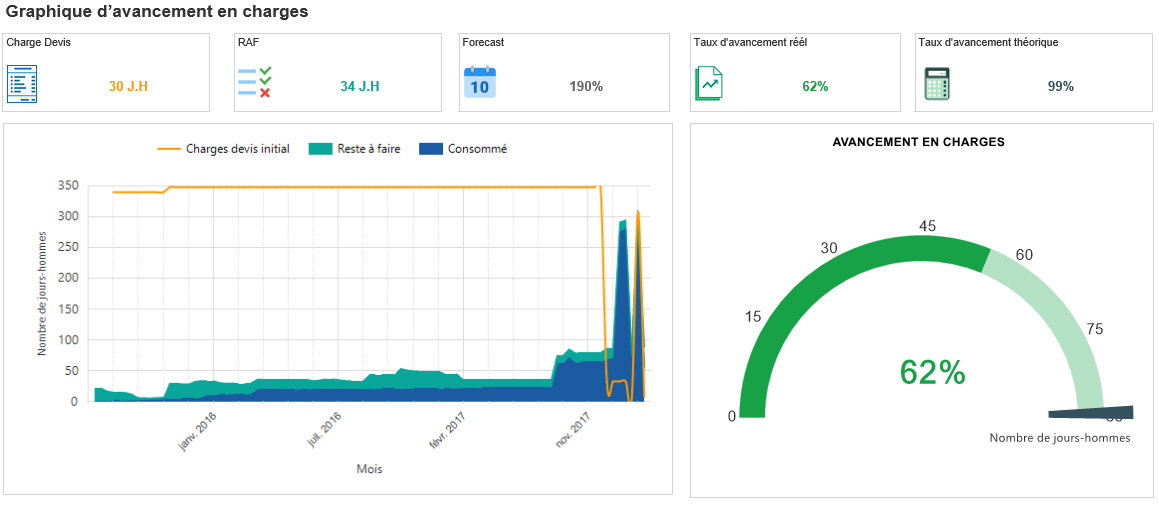
\includegraphics[width=1\textwidth]{images/PPIL-avancement.png}
\caption{PPIL : Graphique d'avancement en charges}
\end{figure}


\begin{figure}[!h]
\centering
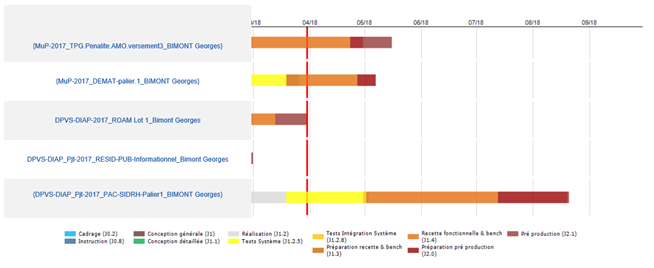
\includegraphics[width=2.5\textwidth]{images/PPIL-Gantt.png}
\caption{PPIL : Gantt des projets contributeurs}
\end{figure}


\section{La qualification}

Une partie de mon stage a été destiné à la qualification : 
\begin{itemize}
    \item Tests fonctionnels
    \item Tests de Non Régression
    \item Plan de tests
\end{itemize}

\subsection{L'importance des tests}

Durant mon stage, j'ai réalisé des tests afin de vérifier le bon fonctionnement des nouvelles fonctionnalités et corrections du projet ainsi que détecter d'éventuels anomalies ou régressions. Ces tests ont été bénéfique pour comprendre PPIL en profondeur. En effet, pour chaque tests, il faut comprendre et manipuler la base de données du projet, consulter les spécifications techniques ou fonctionnelles (SFG, STD) et poser des questions aux différents membres de l'équipe.

Au cours de ces tests, j'ai rencontré plusieurs difficultés : 

\begin{itemize}
    \item comprendre les fonctionnalités à tester
    \item comprendre les principes, la logique de reporting et les différents indicateurs
    \item manipuler une base de donnée complexe
\end{itemize}

A chaque fois, ces tests ont été effectué avant une livraison interne ou une livraison client.

Lors des tests il est important de prendre du recul et de tester d'autres fonctionnalités qui pourrait etre impacté par la correction qu'on est en train de tester afin de détecter d'éventuels régressions.

Tous ces tests ont été réalisé grâce à l'outil HP LM.
        
La validation d'un test c'est prendre la responsabilité de dire qu'on peut livrer l'application. L'étape du test est primordiale, sans celle-ci un bon nombre d'erreurs ne seraient pas détectés.

\subsection{Plan de test}
\begin{figure}[!h]
\centering
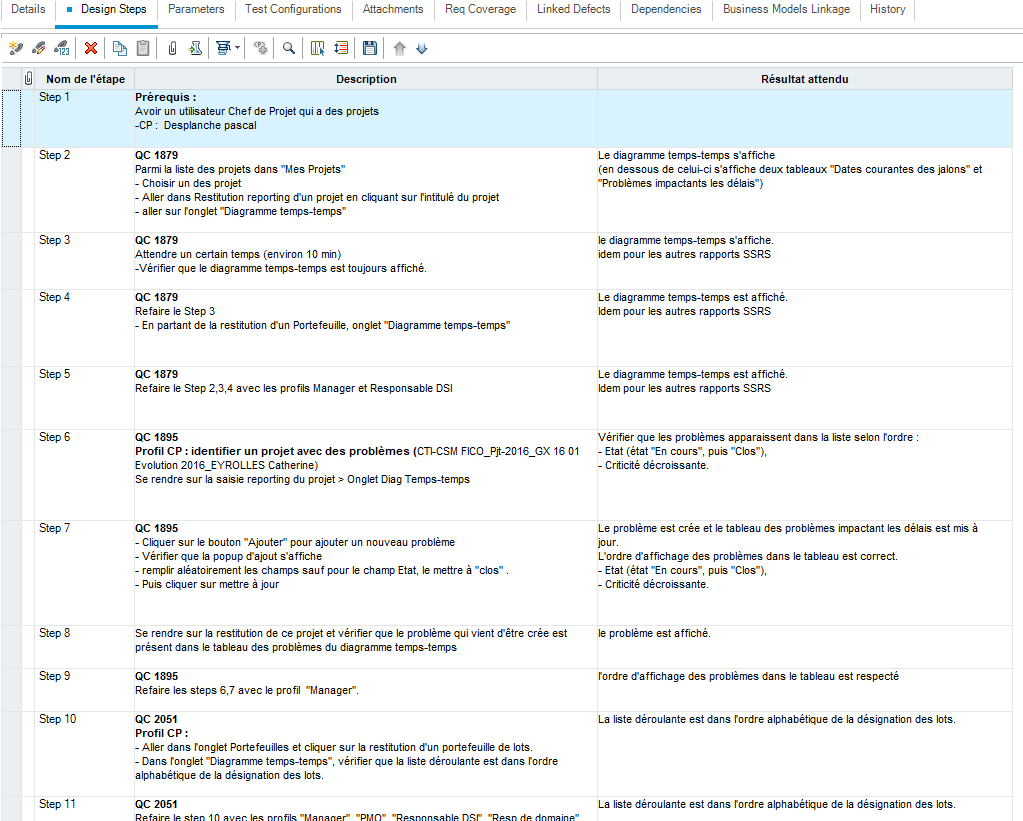
\includegraphics[width=1\textwidth]{images/HPLMplantest.png}
\caption{HP LM : Plan de test}
\end{figure}

\subsection{Un exemple de test réalisé : Les tests de Non Régression (TNR)}

[semaine 11/06]
Avant la livraison de la release 20.06.00. Il a fallut effectuer des tests de non régression.

Je vais décrire ici le test "06-TNR-ReportingRestitutionDuLot". Lors de ce test, j'ai détecté trois Defects. Ce qui a permis d'identifier et corriger 1 anomalie mineure, une anomalie majeur, et une régression majeur. Au cours de ce test de 40 steps, j'ai effectué un grand nombre de requêtes SQL, j'ai du comprendre la logique de calcul ainsi que la logique d'affichage des indicateurs d'avancement d'un projet en fonction des jalons de celui-ci, il a fallu que j'analyse la synchronisation des données projet entre MSP et PPIL.
\subsubsection{Un exemple de difficulté rencontré lors de ce test}

description du step de ce test : 
vérifier que les indicateur de suivi d'avancement des lots sont corrects :
Dans PPIL, dans la partie restitution de l'avancement d'un projet de référence. Dans cette partie il a fallu comprendre comment étaient calculés les indicateurs de restitution pour l'avancement d'un lot. Pour cela j'ai consulté les SFD pour voir les règles de calcul, je suis allé dans le code chercher les procédures stockées, après cela, j'ai fait mes calculs a l'aide de Excel et de SQL, n'ayant toujours pas le même résultat, j'ai demandé des explications à un BA notamment sur la synchronisation des données de MIcrosoft Project dans PPIL(outil utilisé par les CP de la Cnam pour mettre à jour les jalons de leurs projets). Et j'ai analysé une procédure stockée .Grâce à ces explications et à ces analyses j'ai réussi à ajuster ma requête qui n'était pas juste pour ce cas précis de restitution qui importe les projets contributeurs (qui font parti du même PRT Palier).

Pour la partie Avancement en charge
\begin{figure}[!h]
\centering
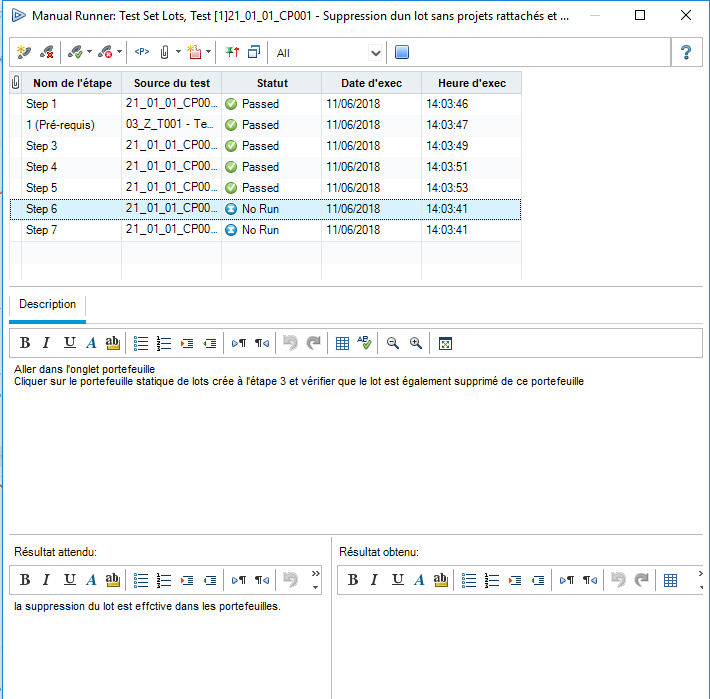
\includegraphics[width=0.8\textwidth]{HPLMtest.png}\\[1cm]
\caption{HP LM : Faire un test}
\end{figure}

\section{Environnement technique du projet}

Toujours pendant la deuxième semaine, j'ai mis en place mon environnement de développement avec Achref (mon SB référent).
le projet PPIL se situe dans un contexte technique Microsoft :

\begin{itemize}
    \item Sharepoint, 
    \item SQLServer, 
    \item .net
    \begin{itemize}
        \item C\#, 
        \item Telerik, 
        \item TypeScrypt, 
        \item Entity Framework, 
        \item SSRS, 
        \item HTML, 
        \item CSS etc).
    \end{itemize}
\end{itemize}

J'ai pu découvrir l'environnement technique.
Nous avons mis Git en place.
IDE = Visual Studio
FONCTIONNEMENT DE TECHNIQUE sprint déploiement MEP des pull request.
\section{Développer au sein de PPIL}
Pendant le mois de Mai
Après un retour client 
J'ai enfin pu commencer à développer
Les développements au sein de PPIL se font en fonction de l'évolution du sprint en cours. Je suis arrivé dans un contexte de CORRECTION D'ANOMALIES. c'est naturellement que des (QC) correction d'anomalies m'ont été attribué.
\subsection{Correction d'anomalies}
Lorsque les BA détectent une anomalie, il l'identifient/la répertorie dans l'outil HPLM. Si l'anomalie est détectée par le client elle sera "taguée" FT.
Les différentes QC sont classées par priorité et importance.
Les FT sont souvent prioritaire par rapport aux anomalies détectés par l'équipe
lot en cours.
\begin{figure}[!h]
\centering
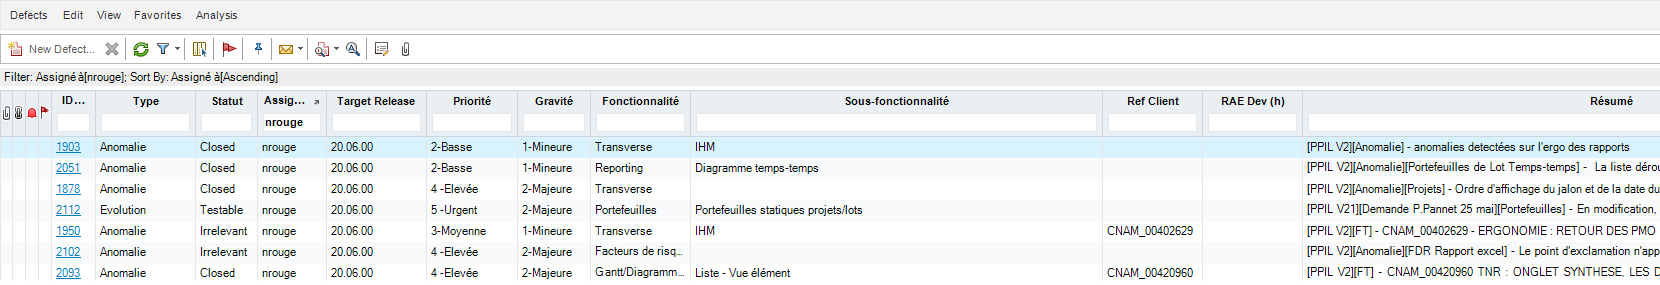
\includegraphics[width=1\textwidth]{images/HPLMliste.png}
\caption{HP LM : mes corrections effectuées pour la release 20.06.00}
\end{figure}
\subsection{Démarche Adoptée}
Au même titre que les SB, j'ai été chargé de corriger des anomalies.
Le référent technique a attribué différentes QC (Anomalies) aux différents SB. 
Les anomalies que j'ai corrigé étaiement toutes différentes et incluaient toutes les technos.
Les anomalies que j'ai corrigé, Par exemple : 
\begin{itemize}
    \item suppression d'un élément qui ne se supprime pas en base
    \item erreur dans le chargement d'une page
    \item bouton "annuler" non présent
    \item ordre ou classement pas correct
    \item direction de page incorrect lors de la consultation...
\end{itemize}
Pour mener à bien ces différentes correction, j'ai du avoir une approche d'ingénierie
il a fallu comprendre l'architecture du programme.
comprendre l'architecture de la BDD.
comprendre les technos.
    se former sur les technos.
comprendre l'anomalie
    et notamment l'ampleur
    pour quel type d'utilisateur 
    dans quel mode (consultation, restitution, 
    dans quel rubrique ( mes prjets, ptf, ...
identifier la provenance du problème
comprendre la logique de développement
comprendre pourquoi le projet a été codé de cette manière
                aller voir les développeurs, 
                le référent technique
                
            identifier les solutions possible
            
            choisir la meilleure façon de faire
                - de façon a modifier au minimum le code
                - la plus optimale
                - sans faire de régression 
                
            respecter les délais, RAE
            aller chercher de l'aide quand il le faut
            respecter les consignes de code

présenter le QUOI et le COMMENT 
l'approche pour arriver au résultat est très important
Après avoir corrigé une anomalie : 
je push ma branche avec git sur le dépot distant
je crée une pull request pour alerter le référent technique.
\begin{figure}[!h]
\centering
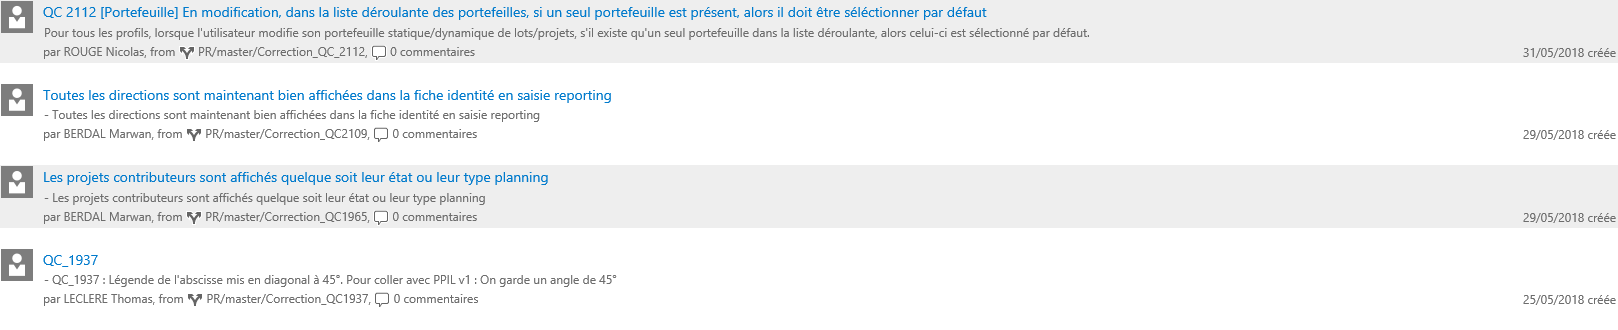
\includegraphics[width=1\textwidth]{images/PullRequest.png}
\caption{Visual Studio Team Foundation : Les Pull Request}
\end{figure}
\subsection{Quelques exemple d'anomalie corrigée}
\subsubsection{PREMEIRE ANO}
Dans la globalité, toutes les anomalies ont été intéressante à corriger.
FT = ano détectée par le client
description de la correction : [Pour le profil CP et Manager]Dans portefeuille, dans la liste déroulante qui apparait lorqu'on veut ajouter les projets ou des lots aux différents portefeuilles, statique, dynamique 4 types de portefeuilles). sélectionner par défaut un portefeuille s'il n'y en a qu'un seul. Ne rien sélectionner par défaut. Pour le responsable DSI, sélectionner par défaut "Mes projet favori" quelque soit le nombre de portefeuille existant.
- Premierement avant de commencer la correction j'ai mis au courant le RT afin de le prévenir que la description du client coprenait des flou / incohérence. Ce qui a été remonté, et il y avait bel et bien un flou.
- ENsuite lors de la correction j'ai un peu galéré au niveau des technos. 
- trouver dans le code ou c'était
\subsubsection{DEUXIEME ANO}
description de l'anomalie : Supression des lots non effective selon certains critères : 
- un lot ne se supprime pas quand il est dans un portefeuille (le lot se supprime visuellement mais pas en base, quand on refresh la page il réapparait)
- un lot ne se supprime pas quand il a des demandes rattachés
- ne se supprime pas quand il n'a pas de projet de référence
Cette anomalie m'a pris plusieurs jours de correction. 
- pendant la correction j'ai détecté une autre ano : un lot sans projet de référence ne s'affiche pas dans un portefeuille. 
- Ano que j'ai corrigé par la suite.
- J'ai proposé une solution
- Lors d'une discussion avec Nicolas (le RT du projet), il a validé ma correction comme étant correcte et en se servant et cohérente.
- Il m'a demandé de refaire une partie de cette correection en modifiant une procédure stockée en SQL plutot que le code. 
préférable de faire comme ça pour la maintenabilité du code et de l'optimisation 
\subsubsection{ANO}
Description de l'ano : en restitution d'un projet, onglet synthèse, quand on remonte sur une semaine précédente, les dates ne sont pas les bonnes. 
IMAGE
Comprendre le fonctionnel. logique des jalons.
Les dates, 
requêtes complexes, 
%%% Local Variables: 
%%% mode: latex
%%% TeX-master: "isae-report-template"
%%% End: 